%%%%%%%%%%%%%%%%%%%%%%%%%%%%%%%%%%%%%%%%%%%%%%%%%%%%%%%%%%%%%%%%%%%%%%%%%%%%%%%%%%%%%%%%%%%
%%
%%   gshs-server-intro by devops members
%%   경기과학고등학교 리눅스 사용자협회
%%   
%%   total supervisor : toadsong8451 (20059 송혁중)
%%   gs20059@gs.hs.kr
%%
%%%%%%%%%%%%%%%%%%%%%%%%%%%%%%%%%%%%%%%%%%%%%%%%%%%%%%%%%%%%%%%%%%%%%%%%%%%%%%%%%%%%%%%%%%%


\RequirePackage[l2tabu, orthodox]{nag} % tells you of any bad LaTeX usage
                                       % must be first thing in class (with the exception of comments)

%% There is one option you should define; oneside or twoside
%% Use twoside for your viva docs (examiners hate long docs they need to carry around)
%% and oneside for the final thing you submit to the library.  Note that margins will
%% change accordingly

\documentclass[twoside]{gshs-server-intro}  % custom gshs


%% **************** (Your) Packages (Start) ******************

% \listfiles % uncomment this to know which packages you are using
              % the list of packages will be in the bottom of the .log file

%% Note that packges may already be loaded from the um (and memoir) classes.
%% Do not add your packages to the template, but rather add them here.

\usepackage{blindtext} %% for some dummy text, remove in your writeup
\usepackage{kotex}
\usepackage{indentfirst}


%% ***************** (Your) Packages (End) *******************


%% **************** (Your) Data (Start) ******************

\title{경기과학고등학교 연구용 서버\\사용 및 관리 설명서}  % use \\ here otherwise you get a justified title
                                                    % note capitalization of the title (only common 
                                                    % words in lower case)
\tagline{version 2.01}                     % tag line
\author{리눅스 사용자 협회}                           % your name
\authorID{GSHS}                           % your University Identifier
\supervisor{20059 송혁중}                             % your supervisor(s) name - no . in Dr
                               % your cosupervisor(s) name - no . in Dr ** OPTIONAL ** 
                                                    % simply comment out the above line if absent
\department{경기과학고등학교}                  % your department (e.g. Artifical Intelligence)
\faculty{정보과학과}                      % your faculty (e.g. ICT)
\degree{M.Sc.\ in Your Degree}                      % the degree you are reading
                                                    % note the \ after the dot, so not to consider it a fullstop
\doctype{설명서}                              % the type of document (fyp, dissertation, thesis)
\degreedate{2022. 5.}                        % when did you submit -- officially after your corrections !
%%\subjectcode{ICS5200}                               % the study unit-code (currently not used)

%% ***************** (Your) Data (End) *******************


%% ******** (Your) Document Settings (Start) *************

% You should have an images directory in every chapX subdir
% NOTE:  Trailing / for subdirs is required.
\graphicspath{{./images/}{./chap1/images/}}   % Paths where to look for images, if defined "images" must always be there as it holds the images in-use by the template.

\makeindex

%% ********* (Your) Document Settings (End) **************

% DOCTOR'S (JP) ORDERS: MAKE SURE TO READ MY TWO BLOG ENTRIES WITH
% CONTENT AND LaTeX TIPS FOR YOUR WRITE-UP.  THESE ARE BASED ON  
% EXAMINER'S FEEDBACK
%
% URLS:
% https://bitsilla.com/blog/2019/03/content-tips-for-your-dissertation-or-project-write-up/
% https://bitsilla.com/blog/2019/01/latex-tips-for-your-dissertation-or-project-write-up/

% end the preamble and start the document

\begin{document}
\frontmatter 
    \maketitle
    \begin{copyrightenv}
\end{copyrightenv}
       
    \begin{originality}
\end{originality}    
    \begin{dedication}
{\large{To The Researchers of Gyeonggi Science High School}}\\[5mm]
Calculation is the best way to prove.
\end{dedication}

        % include a dedication.tex file
    \begin{acknowledgements}
\textbf{
서버의 효율적인 이용을 위해 아래와 같은 규칙들이 있다.}
~\\


\begin{itemize}
 \item 서버는 연구 및 공적 목적으로만 사용 가능하다.
 \item 서버는 함께 사용한다.
 \item 계정명은 반드시 gs00000 (학번)으로 한다.
 \item GPU는 송죽학사를 통해 신청한 자만이 사용할 수 있다.
 \item GPU를 신청하지 않은 상태에서 사용할 시 프로세스가 강제 종료될 수 있다.
 \item 과도한 CPU/GPU/RAM 사용으로 서버에 과부하를 유발하는 프로세스는 강제로 종료될 수 있으며 사용자는 경고를 받을 수 있다. 경고 3회 누적시 GPU 신청이 제한될 수 있다.
 \item 관리자 권한이 없는 계정은 졸업 시 삭제를 원칙으로 한다.
 \item 관리자 계정은 Devops 운영진만이 소유한다.
 \item 허가 없이 reboot 명령어를 사용해서는 안 된다.
 \item 모든 사용자는 자신의 가상환경을 구성해 사용해야 한다.
\end{itemize}~\\



\textbf{
아래는 유용한 링크들이다.}
~\\
\begin{itemize}
 \item 경기과학고등학교 연구용 서버 사용 및 관리 설명서 (\href{https://www.overleaf.com/project/60a1d2365a26a733e5a9b16f}{Overleaf 주소})
 \item 경기과학고등학교 리눅스 사용자 협회 (\href{https://github.com/gshslinuxintro}{Github 주소})
 \item 경기과학고등학교 리눅스 사용자 협회 오픈채팅방 (\href{https://open.kakao.com/o/go6dFeee}{카카오톡 주소})
 \item 현재 연구용 메인서버 IP (\href{http://115.23.235.150}{서버 주소})
 \item 현재 테스트용 서버 IP (\href{http://115.23.235.135}{서버 주소})
\end{itemize}~\\
\end{acknowledgements}   % include an acknowledgements.tex file
    \begin{abstract}
4차 산업혁명이 시작되고, 수많은 데이터가 정보화되어 처리되고 있다. 또, 인공지능과 같은 첨단 프로그램들은 많은 양의 데이터를 빠르게 처리해야 하기에 고성능 컴퓨터를 필요로 한다. 본 설명서는 리눅스 서버를 처음 접하는 정보과학 연구자들을 위해 작성되었다. 특히, 리눅스 서버 이용을 위해 필수적인 ssh, sftp 등의 사용 방법, 공용 서버 사용 규칙, 인공지능 연구를 위해 필수적인 Python, CUDA, TensorFlow, Torch, venv 등의 사용 방법을 다뤘다. 또, 함께 쓰는 공동 연구 환경에서 어떻게 자신의 연구를 해나가야 하는지 방향을 제시했다.~\\


정보과학 연구의 세계는 깊고도 넓기에 연구의 의미와 가치를 잘 이애하고 자신에게 맞는 연구를 하는 것이 중요하다. 연구 방법을 익히고, 다양한 사람들의 연구를 경험해봐야 한다. 저자는 본 설명서를 통해, 서버를 이용한 정보과학 연구에 꼭 필요한 것을들 가려 뽑아 연구의 모든 것을 간명하게 전달하려고 노력했다. 본 설명서가 귀하의 미래를 밝히는 길잡이가 되기를 기원한다.~\\\\
\end{abstract}
\begin{dedication2}
{\large{37기 정보과 일동}}\\[5mm]
2021년 5월 17일, 송죽골에서.
\end{dedication2}\if@openright\cleardoublepage\else\clearpage\fi
    \tableofcontents*\if@openright\cleardoublepage\else\clearpage\fi
    \listoffigures*\if@openright\cleardoublepage\else\clearpage\fi
    \listoftables*\if@openright\cleardoublepage\else\clearpage\fi
    %% will only print what is used ... useful.
%% also acronyms are clickable, which is awesome

\chapter*{List of Abbreviations}
\markboth{List of Abbreviations}{List of Abbreviations}
               
\begin{acronym}\itemsep-20pt\parsep-20pt %% if you remove these spacing params this list becomes huge!
\acro{GSHS}{Gyeonggi Science High School}
\acro{GPU}{Graphic Processing Unit}
\acro{CPU}{Central Processing Unit}
\acro{GUI}{Graphic User Interface}
\acro{CLI}{Command Line Interface}
\acro{CUDA}{Compute Unified Device Architecture}
\acro{CP}{Compute Compatibility}
\acro{UA}{Used Acronym}
\acro{lox}[\ensuremath{LOX}]{Liquid Oxygen}
\acro{lh2}[\ensuremath{LH_2}]{Liquid Hydrogen}
\acro{IC}{Integrated Circuit}
\acro{BUT}{Block Under Test}
\acrodefplural{BUT}{Blocks Under Test}    
\end{acronym}
\if@openright\cleardoublepage\else\clearpage\fi

%% Note: always use \input as you cannot nest \includes (amongst other things)
\definecolor{dkgreen}{rgb}{0,0.6,0}
\definecolor{gray}{rgb}{0.5,0.5,0.5}
\definecolor{mauve}{rgb}{0.58,0,0.82}
\definecolor{codegreen}{rgb}{0,0.6,0} \definecolor{codegray}{rgb}{0.5,0.5,0.5} \definecolor{codepurple}{rgb}{0.58,0,0.82} \definecolor{backcolour}{rgb}{0.95,0.95,0.92}
\makeatletter
\newcommand*\verbfont{%
    \normalfont\ttfamily\hyphenchar\font\m@ne\@noligs}
\makeatother
\lstset{ %
  language=bash,                % the language of the code
  basicstyle   = \color{black}\raggedright\verbfont\footnotesize\selectfont,
  backgroundcolor=\color{backcolour},
  commentstyle=\color{codegreen}
  keywordstyle=\color{magenta},
  numberstyle=\tiny\color{codegray},
  stringstyle=\color{codepurple},  % numberstyle=\footnotesize,          % the size of the fonts that are used for the line-numbers
  stepnumber=2,                   % the step between two line-numbers. If it's 1, each line  % will be numbered
  numbersep=5pt,                  % how far the line-numbers are from the code
  %backgroundcolor=\color{white},      % choose the background color. You must add \usepackage{color}
  showspaces=false,               % show spaces adding particular underscores
  showstringspaces=false,         % underline spaces within strings
  showtabs=false,                 % show tabs within strings adding particular underscores
  frame=single,                   % adds a frame around the code
  tabsize=2,                      % sets default tabsize to 2 spaces
  captionpos=b,                   % sets the caption-position to bottom
  breaklines=true,                % sets automatic line breaking
  breakatwhitespace=false,        % sets if automatic breaks should only happen at whitespace
  title=\lstname,                   % show the filename of files included with \lstinputlisting;
                                  % also try caption instead of title
  %numberstyle=\tiny\color{gray},        % line number style
  %keywordstyle=\color{blue},          % keyword style
  %commentstyle=\color{dkgreen},       % comment style
  %stringstyle=\color{mauve},         % string literal style
  escapeinside={\%*}{*)},            % if you want to add a comment within your code
  morekeywords={*,...}               % if you want to add more keywords to the set
  basicstyle=\ttfamily,
  columns=flexible
}
\pagestyle{gspage}
\mainmatter 
    \chapter{Introduction}

\graphicspath{{./chap1/images/}}   
\textbf{서버는 모두가 함께 사용하는 것입니다.}

\section{Motivation}
경기과학고등학교(\acs{GSHS})에는 고성능 \acs{GPU} 6개, 그리고 40개의 \acs{CPU} 코어를 가진 서버가 있다. 이 서버는 강력하기에 학생들은 자신의 연구에 큰 도움을 받고 있다. 그러나, 그 서버의 무분별한 사용과 관리자 부재로 인해 연구활동에 어려움을 겪게 되었으며 신입생들의 경우 구전으로 전해지는 사용 방법에 의존해야 했다. 이에 문제의식을 느낀 37기 정보과 일동은 경기과학고등학교 리눅스 사용자 협회, 그리고 교내 봉사모둠인 GM을 만들어 서버 사용 및 관리를 체계화하는 한편 본 설명서를 통해 처음 서버를 이용하는 학생들을 돕고자 한다.

\section{Ubuntu}
Ubuntu Linux는 윈도우와 같은 운영체제로, 윈도우와 달리 무료이며 공개 소스이다. 서버에 일반적으로 이용하는 Ubuntu Server는 \acs{GUI}가 없는 Ubuntu로, 마우스 없이 명령줄만으로 제어하는 \acs{CLI} 환경이다. 윈도우의 명령 프롬프트(cmd)와 유사하다.

%\subsection{Showing the Use of Acronyms}

%In the early nineties, \acs{GSM} was deployed in many European countries. \ac{GSM} offered for the first time international roaming for mobile subscribers. The \acs{GSM}’s use of \ac{TDMA} as its communication standard was debated at length. And every now and then there are big discussion whether \ac{CDMA} should have been chosen over \ac{TDMA}.

%If you want to know more about \acf{GSM}, \acf{TDMA}, \acf{CDMA} and other acronyms, just read a book about mobile communication. Just to mention it: There is another \ac{UA}, for testing. 
    
\graphicspath{{./chap2/images/}}
\chapter{Connection}
  
\textbf{이 장은 서버와의 연결, 그리고 파일 송수신 방법을 다룬다.}

\section{SSH를 이용한 서버 접속}
	서버는 학교에 있으므로 원격으로만 이용할 수 있다. 이를 위하여 SSH(Secure SHell)를 쓴다. Putty와 같은 전용 프로그램을 이용해도 되고, OpenSSH를 설치한 후 명령 프롬프트와 같은 환경에서 SSH 명령어를 이용해도 된다. 이 문서에서는 후자를, Windows 10 기준으로 설명하도록 하겠다.\\
	
	먼저 윈도우에서 시작 > 설정 > 앱 > 앱 및 기능에 들어간다.
	\begin{figure}[h]
	\begin{center}
        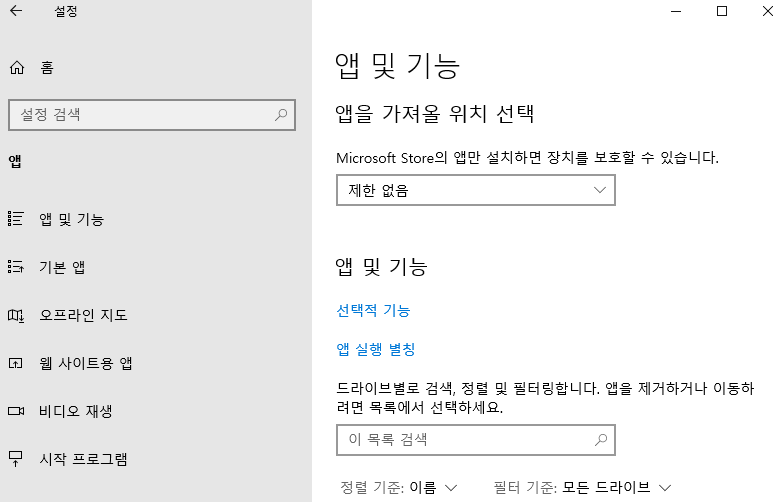
\includegraphics[width=5cm]{ssh1.png}
        \caption{앱 및 기능}
    \end{center}
    \end{figure}
	
	여기서 선택적 기능을 클릭하고 SSH를 검색해 OpenSSH를 찾아 설치한다.
	
	\begin{figure}[H]
	\begin{center}
        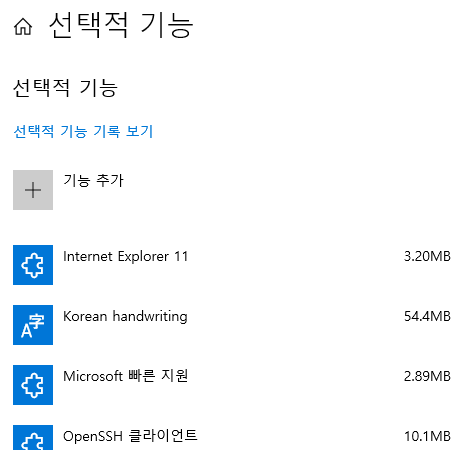
\includegraphics[width=4cm]{ssh2.png}
        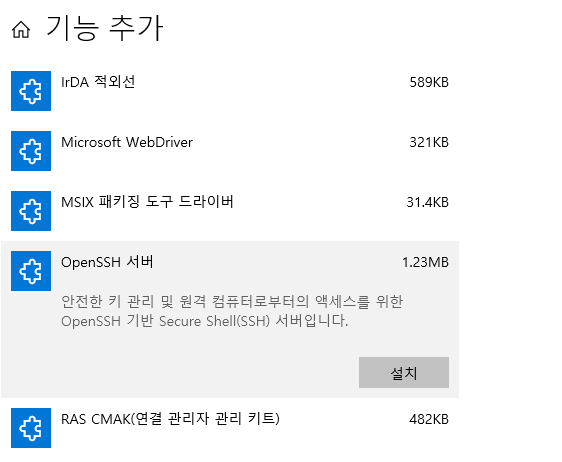
\includegraphics[width=4cm]{ssh3.png}
        \caption{OpenSSH 서버 설치}
    \end{center}
    \end{figure}
    

	경기과학고등학교 연구용 서버는 Ubuntu 18.04로 구성되어 있다. 이 운영체제는 Windows처럼 사용자 이름(username)과 암호(password)가 있어야 한다. 만약 본인이 서버를 이용하고 싶다면 근처의 정보전공 친구에게 사이다를 사주고 계정을 얻어내도록 하자. 일련의 과정을 통해 서버에 접속할 계정명과 암호, 주소와 포트까지 알게 되었다면 다음과 같은 명령어를 통해 서버에 접속할 수 있다. 이후 암호를 입력하면 접속에 성공한 것이다. 참고로 root 계정은 보통 이용하지 않는다.\\
	\begin{lstlisting}
    $ ssh -p [port] [username]@[address]
      ex) ssh -p 22 root@127.0.0.1
    \end{lstlisting}
    
    
   로그인하면 다음과 같은 화면을 볼 수 있다. 참고로 서버는 TUI 환경이기에 접속된 창으로 모든 작업을 수행하게 된다.
    \begin{figure}[H]
	\begin{center}
        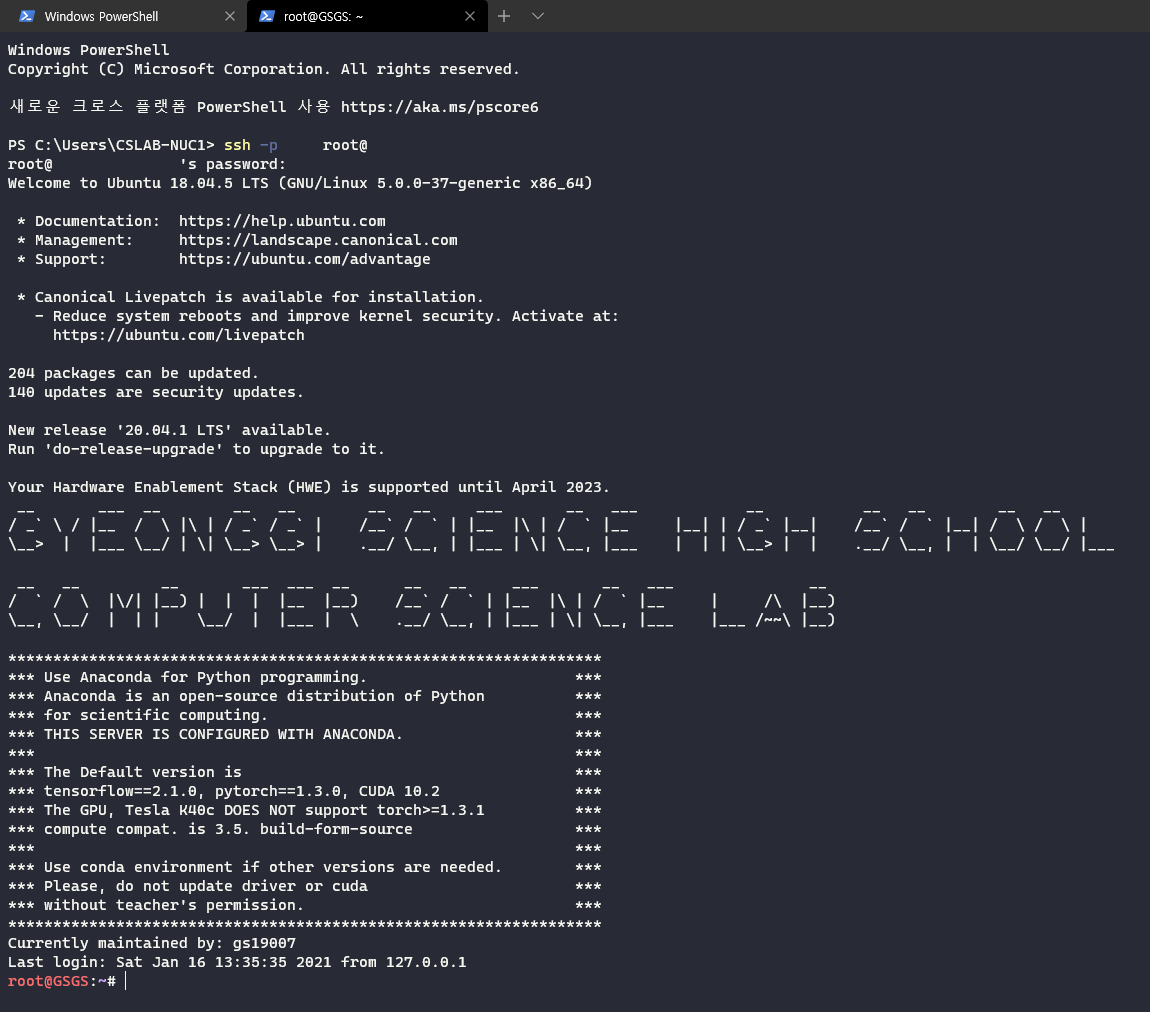
\includegraphics[width=7cm]{ssh5.png}
        \caption{SSH 접속창}
    \end{center}
    \end{figure}
	
\section{SFTP를 이용한 파일 관리}
	SFTP는 SSH File Transfer Protocol의 약어다. 즉, 이미 다룬 SSH 통신을 이용해 파일을 전송하는 것이다. 대표적인 프로그램으로 \href{https://filezilla-project.org/}{FileZilla}가 있다. 파일질라를 설치한 후 좌측 상단 사이트 관리자에서 새 로그인 정보를 만들어 저장하고 연결하면 된다.
	\begin{figure}[H]
	\begin{center}
        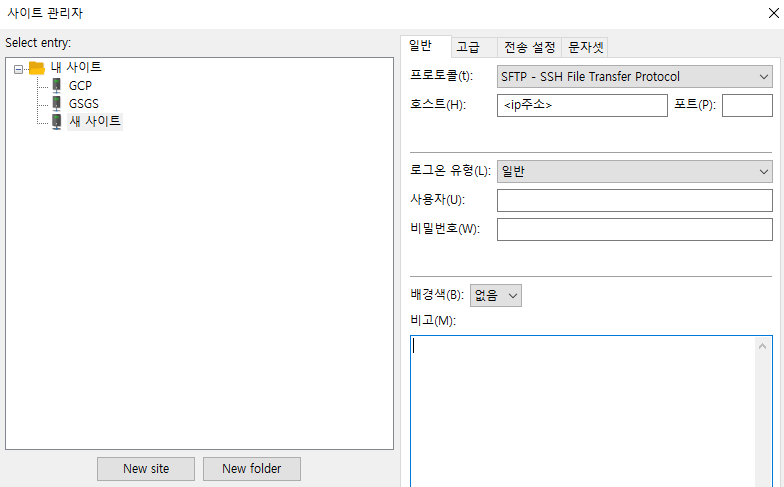
\includegraphics[width=8cm]{sftp2.png}
        \caption{FileZilla 접속}
    \end{center}
    \end{figure}
    접속에 성공하면 화면 양쪽에 파일 탐색기가 생길 것이다. 좌측은 현재 사용자의 컴퓨터이며 우측은 서버다. 이제 사용자는 평소 윈도우 파일 탐색기를 이용하듯 파일을 끌어 옮기거나 다운로드하여 편집할 수 있다. 다만 파일을 다운로드 후 편집하고 다시 업로드를 해야 서버의 파일이 수정된다는 점에 유의해야 한다.
	\begin{figure}[H]
	\begin{center}
        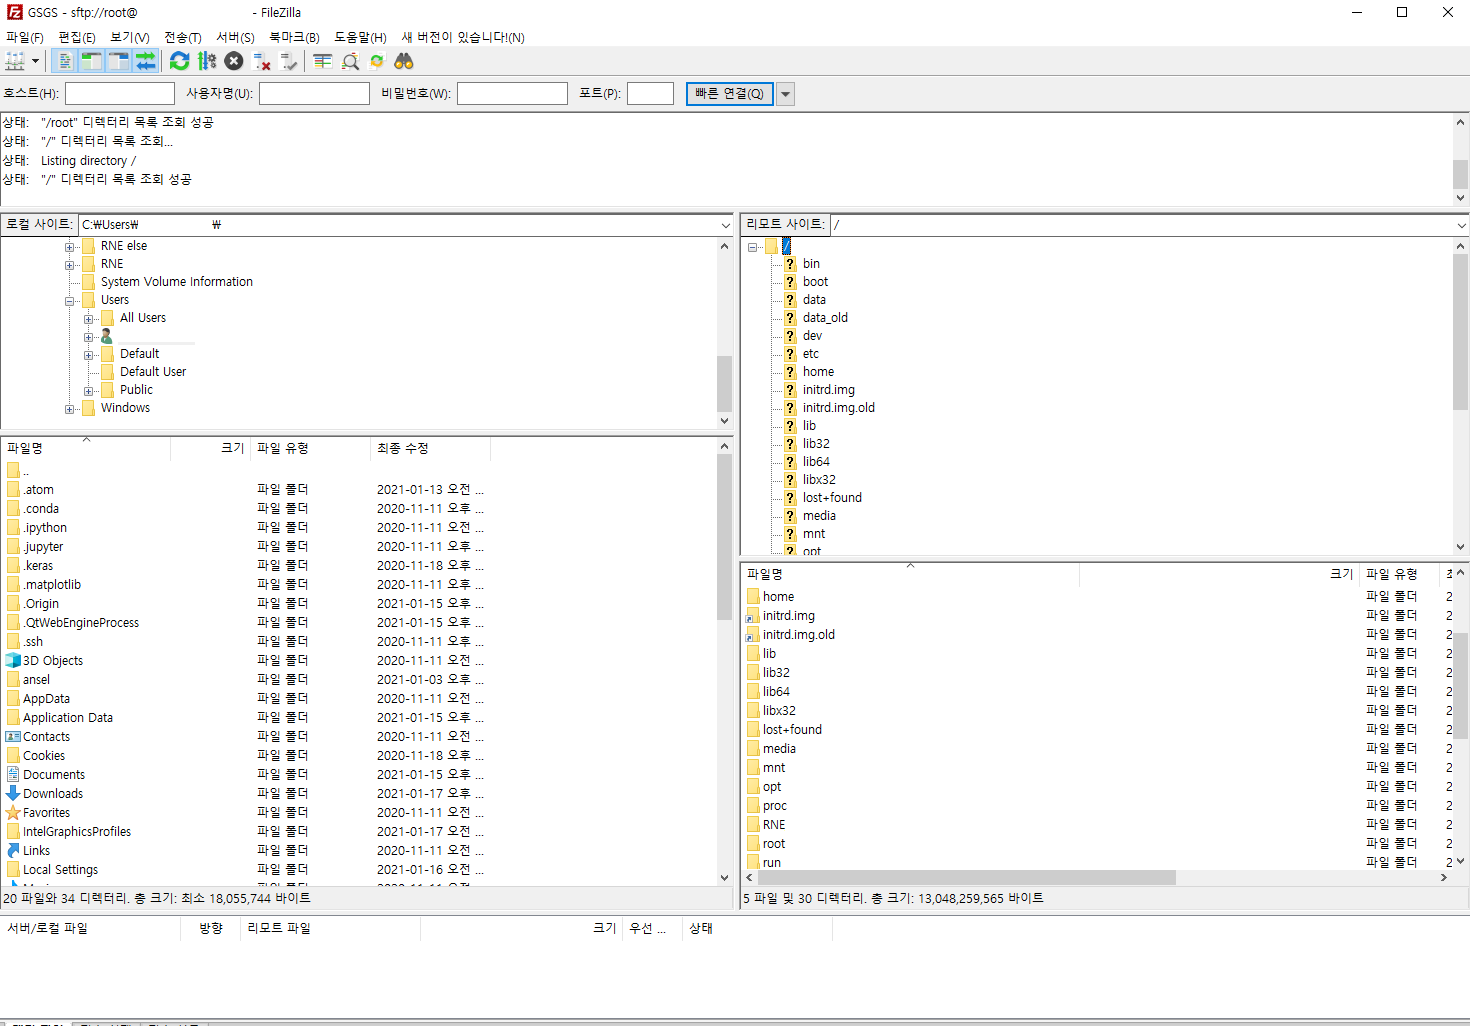
\includegraphics[width=8cm]{sftp3.png}
        \caption{파일질라 접속}
    \end{center}
    \end{figure}
	
    
\graphicspath{{./chap3/images/}} 
\chapter{Command}
\textbf{이 장은 기본 리눅스 명령어를 다룬다.}
\section{파일 관리}
\subsection{절대경로와 상대경로}
절대경로는 /home/gs19000/dir1/dir2와 같은 것이다. 상대경로는 현재 내 위치에서 시작하는 경로다. 즉, 내가 지금 /home/gs19000/dir1에 있다면 여기서 /home/gs19000/dir1/dir2의 상대경로는 그냥 dir2다.
\subsection{디렉토리 및 탐색}
cd 명령어를 사용해서 디렉터리를 탐색할 수 있다. \\ ..은 상위 디렉토리, -은 이전 디렉토리, $\sim$는 홈 디렉토리를 의미한다.
cd (디렉토리)라 치면 해당 디렉토리로 이동된다. 디렉토리를 표현할 때 절대경로, 상대경로 둘 다 가능하며, 실행시 주소쪽 값이 변경된다.
\begin{lstlisting}
    $ cd dir1 입력시
    ~/dir1$ __으로 바뀐다.
    $ cd /home/gs19000/dir1 
    $ cd ..
    $ cd -
    $ cd ~
\end{lstlisting}
\subsection{디렉토리 및 파일 관리}
rm 명령어를 사용해서 파일을 삭제할 수 있다.\\
rm (file) : 해당 파일을 삭제한다. rm -r (dir) : 해당 디렉토리를 삭제한다.
또한, mkdir 명령어를 사용해서 디렉터리를 만들 수 있다.\\
mkdir (dir) : 해당 이름의 디렉토리가 존재하지 않을 경우 새로 dir이름의 디렉터리를 생성한다.\\


다음으로 cp, mv 명령어를 통해 파일을 옯기거나 복사할 수 있다.\\
cp (file1) (file2) : file1의 이름을 file2 이름으로 바꾸어 복사한다.(file1은 삭제되지 않음 file2가 이미 존재할 경우 덮어씌워진다)\\
cp -r (dir1) (dir2) : dir1이름의 디렉토리를 dir2 디렉토리 내부에 복사한다.(dir1은 반드시 존재해야 하며 dir2는 존재하지 않을 경우 새로 만들어진다)\\
mv (file1) (file2) : file1의 이름을 file2로 바꾼다.(file2가 이미 존재할 경우 덮어씌워진다)\\
mv (dir1) (dir2) : dir1의 이름을 dir2로 바꾼다.(dir1은 반드시 존재해야 하며 dir2가 존재할 경우 dir2 내부에 dir1 파일을 이동시킨다.)\\
마지막으로, cat을 이용해 내용을 읽어올 수 있다. cat (file1) : file1의 내용을 불러온다.
    \begin{lstlisting}
    $ rm file1
    $ rm -r dir1
    $ mkdir dir2
    $ cp file1 file2
    $ cp -r dir1 dir2
    $ mv file1 file2
    $ mv dir1 dir2
    $ cat file3.txt
    \end{lstlisting}
\section{기타 기능}
\subsection{프로세스 관리}
htop을 이용해 실행중인 프로세스를 확인할 수 있다. kill, pkill을 통해 프로세스를 제거할 수 있다.
    \begin{lstlisting}
    $ htop
    $ kill -9 <pid>
    \end{lstlisting}
\subsection{권한 관리}
chmod를 이용해 권한을 관리할 수 있다. 권한에 대한 자세한 정보는 ...
    \begin{lstlisting}
    $ sudo chmod 777 file1
    \end{lstlisting}
\subsection{Vim}
기본 메모장과 같다. 우분투 서버를 지속적으로 다룰 생각이 있다면 Vim 에디터에 익숙해질 필요가 있다. 먼저, vim 에디터를 사용하여 파일을 수정하기 위해서는 vim 에디터를 실행해야 한다. vim 에디터는 다음과 같은 명령어를 통해 실행할 수 있다.
    \begin{lstlisting}
    $ vim filename
    \end{lstlisting}
위와 같이 vim 에디터를 통해 파일을 열게 되면 다음과 같은 화면이 나타난다.

\begin{figure}[H]
	\begin{center}
        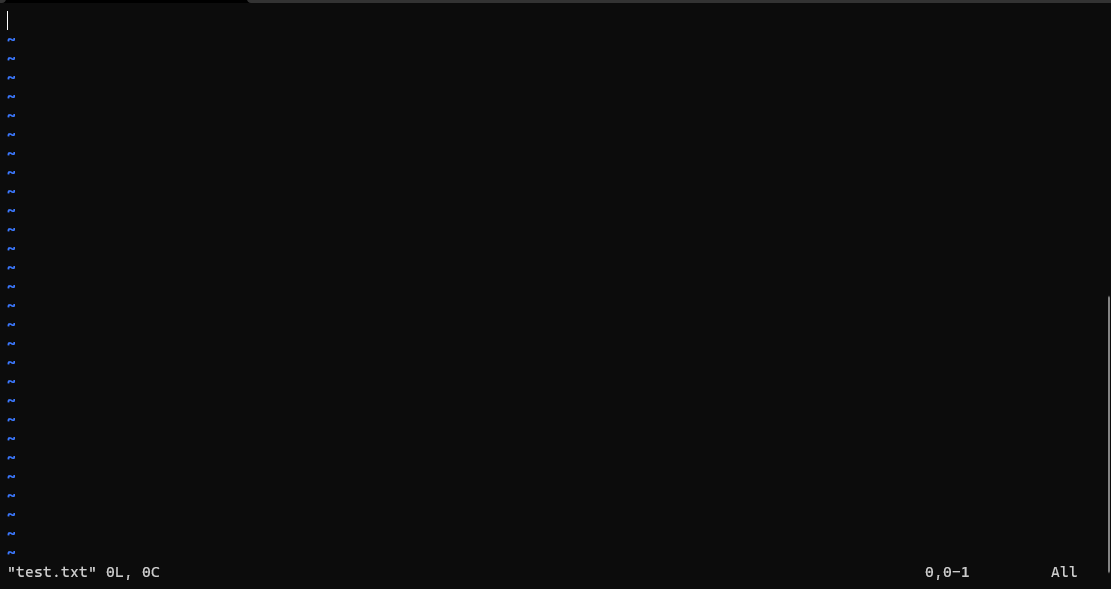
\includegraphics[width=0.8\linewidth]{chap3/images/vim.png}
        \caption{vim 에디터 실행 화면}
    \end{center}
\end{figure}

그런데 이 상태에서 무언가를 입력하려 하면 아마 파일이 수정되지 않을 것이다.\\
왜냐하면 vim 에디터는 수정 모드가 아니라면 파일의 내용을 수정할 수 없기 때문이다.\\
vim 에디터에서 수정모드로 변환하는 방법은 간단하다. i를 입력하면 수정모드로 변환되며, 만약 수정모드를 다시 끄고 싶다면 ESC 키를 누르면 수정모드가 종료된다.\\
수정모드가 아닌 상태에서는 여러 가지 단축키와 커맨드를 통해 여러 기능을 사용할 수 있는데, 이 문서에서는 자주 사용하는 기능의 단축키만을 다룰 것이다. 아래 단축키들을 자주 사용하므로 미리 숙지해놓자.\\

\subsubsection{이동}
\paragraph{기본 이동}
\begin{itemize}[$\bullet$]
    \item h,j,k,l : 좌,하,상,우 커서 이동
    \item - : 줄의 처음 위치로 이동
    \item gg : 맨 위로 커서 이동
    \item Shift + g : 맨 아래로 커서 이동
\end{itemize}
\paragraph{단어 단위로 이동}
\begin{itemize}[$\bullet$]
    \item w : 단어의 시작 위치로 커서 이동 (forward 방향)
        \begin{itemize}[Ex)]
            \item 3w : 세 단어 앞으로 커서 이동
        \end{itemize}
    \item e : 단어의 마지막 위치로 커서 이동 (forward 방향)
    \item b : 단어의 시작 위치로 커서 이동 (backward 방향)
    \item ge : 단어의 마지막 위치로 커서 이동 (backward 방향)
\end{itemize}
\paragraph{한 문장 내에서의 이동}
\begin{itemize}[$\bullet$]
    \item \^ : 문장 맨 앞으로 커서 이동
    \item \$ : 문장 맨 뒤로 커서 이동
\end{itemize}
\paragraph{대략적인 위치로 이동}
\begin{itemize}[$\bullet$]
    \item Shift + h : 현재 보이는 페이지를 기준으로 맨 위로 커서 이동
    \item Shift + m : 현재 보이는 페이지를 기준으로 중간 라인으로 커서 이동
    \item Shift + l : 현재 보이는 페이지를 기준으로 가장 아래로 커서 이동
\end{itemize}
\paragraph{페이지 이동}
\begin{itemize}[$\bullet$]
    \item Ctrl + f : 다음 페이지의 첫 줄로 커서 이동
    \item Ctrl + b : 다음 페이지의 마지막 줄로 커서 이동
    \item Ctrl + d : 페이지의 절반 크기만큼 아래로 커서 이동
    \item Ctrl + u : 페이지의 절반 크기만큼 위로 커서 이동
\end{itemize}
\paragraph{원하는 줄 번호로 한번에 이동}
\begin{itemize}[$\bullet$]
    \item :[number] : [number]행으로 이동
        \begin{itemize}[Ex)]
            \item :3 : 3번째 줄로 이동. 줄 번호는 1부터 시작한다.
        \end{itemize}
\end{itemize}
\paragraph{\{\} 기준으로 이동}
\begin{itemize}[$\bullet$]
    \item ]] : \{로 커서 이동 (forward 방향)
        \begin{itemize}[$\circ$]
            \item 없으면 페이지의 맨 아래로 커서 이동
            \item \{은 가장 상위의 블록을 감싸고 있는 문자만 찾는다.
        \end{itemize}
    \item[$\bullet$] [[ : \{로 커서 이동 (backward 방향)
    \item ][ : \}로 커서 이동 (forward 방향)
        \begin{itemize}[$\circ$]
            \item 없으면 페이지의 맨 아래로 커서 이동
            \item \}은 가장 상위의 블록을 감싸고 있는 문자만 찾는다.
        \end{itemize}
    \item[$\bullet$] [] : \}로 커서 이동 (backward 방향)
    \item \% : \{\}나 ()에서 현재 괄호의 짝으로 커서 이동
\end{itemize}

\subsubsection{편집}
\paragraph{삽입 관련 단축키}
\begin{itemize}[$\bullet$]
    \item i : 현재 커서가 위치한 문자의 앞에 insert 하기
    \item I : 현재 커서가 위치한 줄 맨 앞에 insert 하기
    \item a : 현재 커서가 위치한 문자의 뒤에 insert 하기
    \item A : 현재 커서가 위치한 줄 맨 뒤에 insert 하기
    \item O : 현재 커서가 위치한 줄 바로 윗줄에 insert 하기
    \item o : 현재 커서가 위치한 줄 바로 아랫줄에 insert 하기
\end{itemize}
\paragraph{삭제/잘라내기 및 수정 관련 단축키}
\begin{itemize}[$\bullet$]
    \item dd : 커서가 위치한 줄 잘라내기
    \item dw : 커서가 위치한 곳부터 단어의 마지막까지 잘라내기
    \item Shift + d : 커서가 위치한 곳부터 줄의 끝까지 잘라내기
    \item x : 커서가 위치한 문자 잘라내기
    \item Shift + x : 커서가 위치한 문자 바로 앞에 있는 문자 잘라내기
    \item s : 커서가 위치한 문자 잘라내고 insert 하기
    \item cc 또는 Shift + s : 커서가 위치한 줄 전체 잘라내고 insert 하기
    \item cw : 커서가 위치한 곳부터 단어의 마지막까지 잘라내고 insert 하기
    \item Shift + c : 현재 커서의 위치부터 줄의 끝까지 잘라내고 insert 하기
    \item r + [변경할 문자] : 커서가 위치한 문자 하나 수정하기
        \begin{itemize}[Ex)]
            \item 4rx : 현재 커서 이후 4개의 글자를 x로 수정한다.
        \end{itemize}
\end{itemize}
\paragraph{복사/붙여넣기 관련 단축키}
\begin{itemize}[$\bullet$]
    \item yl : 현재 커서가 위치한 문자 하나만 복사하기
        \begin{itemize}[Ex)]
            \item 3yl : 현재 커서 이후 3개의 문자를 복사한다.
        \end{itemize}
    \item yy : 현재 커서가 위치한 줄 복사하기
    \item yw : 현재 커서의 위치부터 단어가 끝나는 위치까지 복사하기
    \item y : 블럭 단위로 체크한 내용(비주얼 모드 이용) 복사하기 - 한 문자만 복사 X
        \begin{itemize}[Ex)]
            \item[Ex)] [number] + y : 커서가 위치한 줄부터 [number]만큼의 줄 복사하기
            \item y\$ : 커서가 위치한 곳부터 줄의 마지막까지 복사하기
        \end{itemize}
    \item p : 복사한 것을 붙여넣기. 단어를 복사한 경우 커서가 위치한 곳에 붙여넣고, 행 단위를 복사한 경우 커서가 위치한 줄 다음 줄에 붙여넣는다.
    \item Shift + p : 복사한 것을 앞에 붙여넣기. 단어를 복사한 경우 커서가 위치한 곳 앞에 붙여넣고, 행 단위를 복사한 경우 커서가 위치한 줄 바로 윗줄에 붙여넣는다.
    \item[$\bullet$] [number] + p : [number] 만큼 붙여넣기를 반복.
\end{itemize}

이외에도 다양한 단축키가 있으니, 위 목록에 없는 단축키를 안다면 추후 추가 바람.

\subsection{Pipeline}
파이프라인을 통해 출력값에서 원하는 문자열을 확인할 수 있다. 보통 아래와 같이 |와 grep을 이용해 사용한다. 아래의 경우 file2.txt를 출력하는데, 그중 "abc"가 포함된 부분을 찾는 것이다.
    \begin{lstlisting}
    $ cat file2.txt | grep abc
    \end{lstlisting}

    
\graphicspath{{./chap4/images/}}  
\chapter{Environments}

\textbf{이 장은 기본 연구 환경을 다룬다.}
\section{주의사항}
\begin{itemize}
 \item \textbf{sudo reboot은 그 어떠한 경우에도 사용하면 안 된다.} 새로운 프로그램을 설치하는 등 작업 도중 블로그 글을 따라쓰게 될 수 있는데, 그중에 reboot 명령어가 있으면 건너뛰자. 타인의 프로세스가 비정상적으로 종료될 위험이 크다.
 \item \textbf{모든 사용자는 반드시 가상환경을 구성하고, 그 가상환경 내에 여러가지 연구에 필요한 프로그램들을 설치해 사용해야 한다.} 이렇게 하면 관리자 권한 없이 원하는 대로 프로그램의 버전이나 설정을 바꿀 수 있다.
\end{itemize}


\section{간편 설치}
\label{easy}
관리자가 미리 만들어 둔 계정의 폴더를 복사한다.
\begin{lstlisting}
    $ cp -r /home/sampleUser/* ~/
\end{lstlisting}
이 방법을 사용하면 \ref{venv}와 \ref{jupyter}로 향하면 된다.~\\\\

\section{가상환경 설치 및 이용}
\label{venv}
만약 가상환경을 추가로 설치하려 하거나 \ref{easy}의 간편 설치를 이용하지 않았다면 다음 명령어로 가상환경을 설치하자. 
\begin{lstlisting}
    $ virtualenv venv
    $ virtualenv venv --python=python3.6
\end{lstlisting}
여기서 3.5 대신 원하는 다른 버전을 다운받아도 된다. \\
~\\


이후 가상환경을 사용할 때에는 다음 명령어를 사용하면 된다.
\begin{lstlisting}[language=bash]
    $ source ~/venv/bin/activate
\end{lstlisting}
\begin{figure}[H]
	\begin{center}
        
\includegraphics[width=0.6\linewidth]{venv}
        \caption{활성화된 venv 환경}
    \end{center}
    \end{figure}
\section{Jupyter Notebook 설치}
\label{jupyter}
가상환경을 켠 상태로 다음 명령어를 입력하자.
\begin{lstlisting}
    $ pip3 install jupyter
\end{lstlisting}
설치가 제대로 되었는지를 확인하기 위해 다음 명령어를 입력하여 Jupyter Notebook 버전을 확인하자.
\begin{lstlisting}
    $ jupyter --version
\end{lstlisting}

\begin{figure}[H]
	\begin{center}
        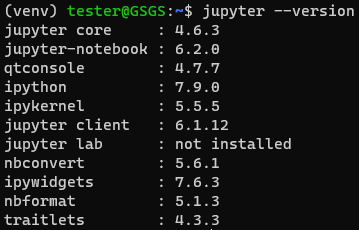
\includegraphics[width=0.4\linewidth]{jupyter_version}
        \caption{Jupyter Notebook 버전 확인}
    \end{center}
\end{figure}

다음 명령어를 입력하여 $\sim$/.jupyter 디렉토리에 접근하자.
\begin{lstlisting}
    $ cd ~/.jupyter
\end{lstlisting}
만약 해당 디렉토리가 존재하지 않는다면, 다음 명령어를 입력하여 해당 디렉토리를 생성한 후 해당 디렉토리에 접근하면 된다.
\begin{lstlisting}
    $ mkdir ~/.jupyter
\end{lstlisting}
이제 다음 명령어를 이용하여 config 파일을 생성하자.
\begin{lstlisting}
    $ jupyter notebook --generate-config
\end{lstlisting}

\begin{figure}[H]
	\begin{center}
        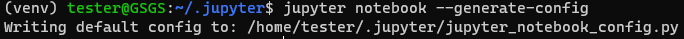
\includegraphics[width=0.8\linewidth]{jupyter_config_generation}
        \caption{Jupyter Notebook config 파일 생성}
    \end{center}
\end{figure}

이제 $\sim$/.jupyter 디렉토리에 jupyter\_notebook\_config.py라는 파일이 생성되었을 것이다. 해당 파일의 내용을 지우고 다음 내용을 입력하자. 단, username에는 자신의 아이디를, student\_number에는 자신의 학번을 입력한다.
\begin{lstlisting}
    c = get_config()
    c.NotebookApp.allow_origin='*'
    c.NotebookApp.notebook_dir='/home/username'
    c.NotebookApp.ip='115.23.235.135'
    c.NotebookApp.port=student_number
    c.NotebookApp.open_browser=False
\end{lstlisting}
이제 jupyter notebook을 실행시키기 위해 다음 명령어를 입력하자.
\begin{lstlisting}
    $ jupyter notebook --config ~/.jupyter/jupyter_notebook_config.py
\end{lstlisting}
이제 터미널 창에 뜨는 url을 복사하여 접속하면 jupyter notebook을 사용할 수 있다.\\

\begin{figure}[H]
	\begin{center}
        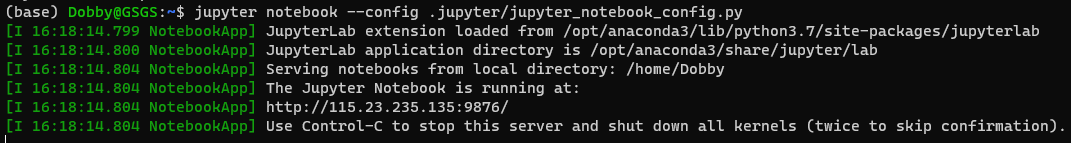
\includegraphics[width=0.6\linewidth]{jupyter_notebook_running}
        \caption{Jupyter Notebook 실행 모습}
    \end{center}
\end{figure}

\begin{figure}[H]
	\begin{center}
        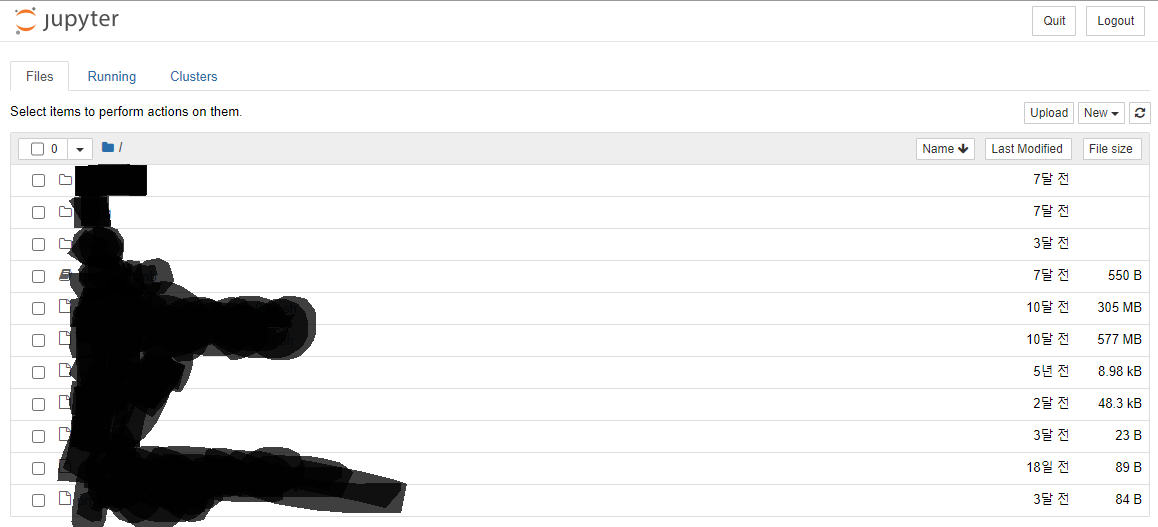
\includegraphics[width=0.8\linewidth]{jupyter_notebook_display}
        \caption{Jupyter Notebook 화면}
    \end{center}
\end{figure}

터미널 창의 세션이 종료되어도 jupyter notebook이 계속 실행되도록 하려면 nohup 명령어를 이용하면 된다.
\begin{lstlisting}
    $ nohup jupyter notebook --config ~/.jupyter/jupyter_notebook_config.py
\end{lstlisting}
\section{tensorflow 설치(선택)}
가상환경을 켠 상태로 다음 명령어를 입력하자.
\begin{lstlisting}
    $ pip3 install --upgrade tensorflow
\end{lstlisting}
\section{CUDA 설치}
만약 서버에 없는 \acs{CUDA}가 필요하다면 관리자에게 문의해야 한다. 이후 자신의 환경변수에 설치된 특정 버전의 \acs{CUDA}를 추가하면 된다.~\\


관리자는 \acs{CUDA}의 정상 작동을 위해 노력해야 한다. 자세한 내용은 Chapter 6 참고.\\
    
\section{쉘 바꾸기(선택)}
만약 계정이 불가피하게 useradd 명령어로 생성되었거나 프로파일이 손상된 경우 bash가 자동으로 활성화되지 않을 수 있다. 사실 쉘에는 sh, bash 등이 있는데, 계정명이 초록색이 아니고 경로가 표시되지 않는다면 쉘이 sh로 설정이 되어있을 수 있다. bash가 여러가지 좋은 기능(위 아래 방향키로 이전 명령 불러오기 등)이 있으므로 다음 명령어를 쳐서 bash로 쉘을 바꿔주자.
\begin{lstlisting}
    $ chsh -s /bin/bash
\end{lstlisting}
이후 서버와의 연걸을 한 번 끊었다가 재접속했을 때 아래처럼 \$ 옆에 사용자명이 뜨면 성공한 것이다.
\begin{figure}[H]
	\begin{center}
        
\includegraphics[width=5cm]{bash}
        \caption{bash로 변경}
    \end{center}
\end{figure}
현재 서버에서 bash 쉘을 사용하는 상태에서 GPU를 사용하는 프로그램을 실행시키는 경우, GPU에 메모리만 할당되고 GPU를 사용하지 않는 현상이 종종 나타나고 있으니 만약 bash 쉘을 사용하는데 GPU 사용량이 이상할 만큼 저조하다면, 이를 한 번 의심해보자. 해당 프로그램을 실행시킬 때에만 bash를 사용하지 않으면 이러한 문제를 해결할 수 있다.
    \graphicspath{{./chap6/images/}}  
\chapter{Admin}
\textbf{이 장은 관리자 작업과 관련된 것들을 다룬다.}

\section{공지}
서버에는 여러 학생들의 연구 및 논문 데이터가 있다. 그러므로 서버에서의 중대한 작업이 진행될 경우 사전에 공지하여 백업하도록 하는 것이 바람직하다. 리눅스 사용자 협회 오픈채팅방 등을 이용하면 된다.
\subsection{유저 관리}
adduser를 이용해 유저를 생성할 수 있다. usermod를 이용해 유저의 그룹을 관리할 수 있다. su를 이용해 사용자를 바꿀 수 있다. useradd를 사용할 경우 유저의 홈 디렉트리, bash 쉘 등이 생성되지 않으므로 adduser의 사용을 권장한다.
    \begin{lstlisting}
    $ adduser gs21000
    $ usermod -aG GROUP gs21000
    $ su gs20000
    \end{lstlisting}
\section{초기화}
서버에 중대한 문제가 발생하여 해결이 불가하거나 심히 어려운 경우 초기화가 그 해결책이 될 수 있다. 본 문서는 Ubuntu Server 20.04.2 LTS를 기반으로 작성되었다.
\subsection{설치디스크 준비}
\begin{enumerate}
    \item 2GB 이상의 USB 준비
    \item 우분투 이미지 사이트\href{https://releases.ubuntu.com/20.04/}{(링크)}에서 Ubuntu Server 20.04 준비한다. 원하는 버전을 준비하면 된다. 중요한 것은 LTS 버전을 다운로드해야 된다는 것이다. 
    \item Rufus\href{https://rufus.ie/}{(링크)} 준비
    \item Rufus 실행 후 준비한 iso 선택
    \item 준비한 USB를 선택하고 '시작' 클릭 (iso 우선 모드는 큰 상관이 없다. 
\end{enumerate}
\subsection{기타 OS 설치}
방법은 동일하다. 현재 관리자 송혁중은 OPENSUSE에 빠져 상업용 Opensuse를 무료로 사용할 수 있는 권한까지 받아 학교 서버에 설치할 수 있었지만 호환성 문제로 하지 않았다. 그러니 다른 OS는 추천하지는 않는다. 다른 OS를 깔았다가 모든 학생들이 반발하는 모습을 볼 수 있을 것이다. 특히나 데비안 계열에서 다른 계열로 변경하는 것은 비추천한다...
\subsection{Ubuntu 설치}
연구용 서버는 SRC 7층 서버실에 위치해 있다. 먼저 7층 교무실에 계시는 정덕교 선생님이나 박종화 선생님께 서버 초기화를 위해 왔음을 알여야 한다. 

테스트용서버(구서버)는 서버실에서 가장 가까운 서버렉의 제일 아래에 있다. 후면에 USB와 VGA 단자가 있고 안쪽에는 키보드, 마우스와 모니터가 있으므로 연결하여 작업하면 된다. 먼저 전원 버튼을 꾹 눌러 종료시킨 뒤 다시 눌러 시스템을 시작한다. 이후 바이오스 창이 나올 때 F2 또는 Del 키를 누르면 부팅 디스크를 선택할 수 있게 된다.
메인서버(신서버, 115.23.235.150)은 서버실의 가장 가까운 서버렉의 위에서 2번째 칸에 위치한다. gpu 10장이 들어가기 위한 것 같아보이는 서버가 신서버이다. 마찬가지지만 usb 단자가 앞면에 위치하고 있다. 
이후 설치 과정을 따라하면 된다. 이때 OpenSSH-Server를 설치하는 것을 추천한다. 또, 중간에 네트워크를 설정하는 창이 나오면 설정표\href{https://github.com/gshslinuxintro/Server-Configuration/blob/main/Network.md}{(비공개 링크)}를 보고 정덕교 선생님께 여쭤보며 작성하면 된다. 신서버를 처음 설치할때는 22.04 버전을 설치하였지만 호환성이 맞지 않는 패키지가 많았으므로 이를 해결하기 위해서 20.04로 다운그레이드를 진행하였다. 버전 업그레이드는 추천하지 않는다. (cuda의 지원 속도가 매우 느린 편)

\section{Drivers}
\textbf{이 Section은 어떤 드라이버도 깔려 있지 않은 상태에서의 설치 상황을 다룬다. 설치과정에서 자동으로 driver를 설치할 수는 있지만 추천하지 않는다.}

먼저 아래 명령어를 통해 현재 설치된 GPU에 적합한 드라이버를 찾을 수 있다.
\begin{lstlisting}
    $ ubuntu-drivers devices
\end{lstlisting}
이후 그중 하나를 골라(recommended) 설치하면 된다.
\begin{lstlisting}
    $ sudo apt install nvidia-driver-XXX (숫자)
\end{lstlisting}
적용하려면 재부팅이 필요하다.
\begin{lstlisting}
    $ sudo reboot
\end{lstlisting}
Nvidia-smi를 통해 설치를 확인할 수 있다.
\begin{lstlisting}
    $ nvidia-smi
\end{lstlisting}
\begin{figure}[H]
	\begin{center}
        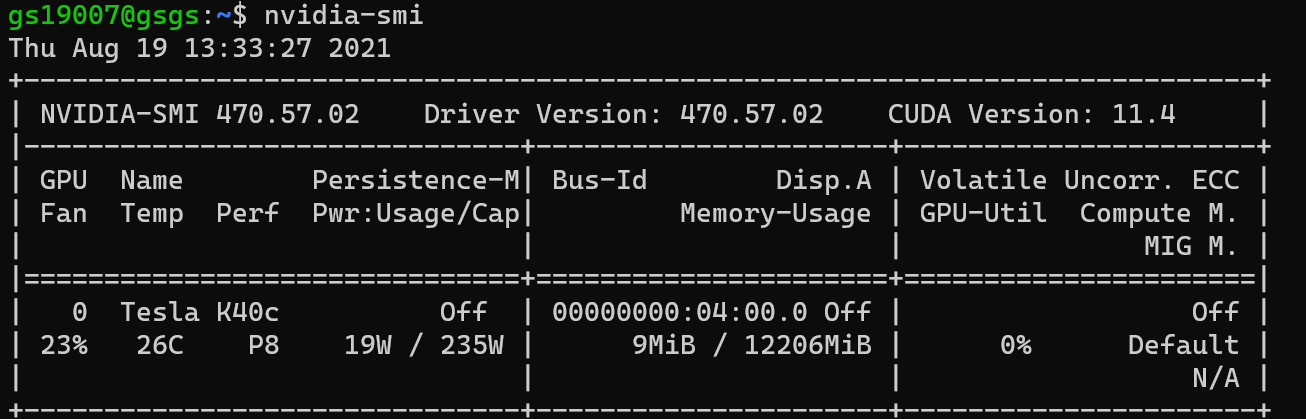
\includegraphics[width=5cm]{nvidia-smi}
        \caption{nvidia-smi}
    \end{center}
\end{figure}
여기서 CUDA Version은 권장 사항으로, 실제 CUDA 버전 및 설치 유무와는 상관 없다.


\section{CUDA 및 cuDNN}
\subsection{CUDA 설치}
기본적으로 알아야 할 사실은 CUDA가 라이브러리라는 것이다. 그렇기에 여러 CUDA 버전을 동시에 설치할 수 있다. 또, debian package로 설치하지만 않았다면 다음 명령어를 통해 쉽게 제거할 수 있음을 기억하자.
\begin{lstlisting}
    $ sudo rm -rf /usr/local/cuda*
\end{lstlisting}

CUDA 설치를 위해서는 gcc가 필요하다.
\begin{lstlisting}
    $ sudo apt-get install build-essential
\end{lstlisting}
이후 CUDA 설치를 위해 먼저 Nvidia Developer 사이트\href{https://developer.nvidia.com/cuda-toolkit-archive}{(링크)}에 들어간다.

여기서 현재 서버의 상황에 맞는 버튼들을 누른다. 참고로 CUDA 12 이후 버전들은 점진적으로 Compute Compatability가 3.x대인 GPU들에 대한 지원을 제한하고 있는데, 연구용 서버에 장착된 GPU인 Tesla K40c의 Compute Compatability는 3.5다. 따라서 11.2 이하 버전의 설치를 권장한다.
\begin{figure}[H]
	\begin{center}
        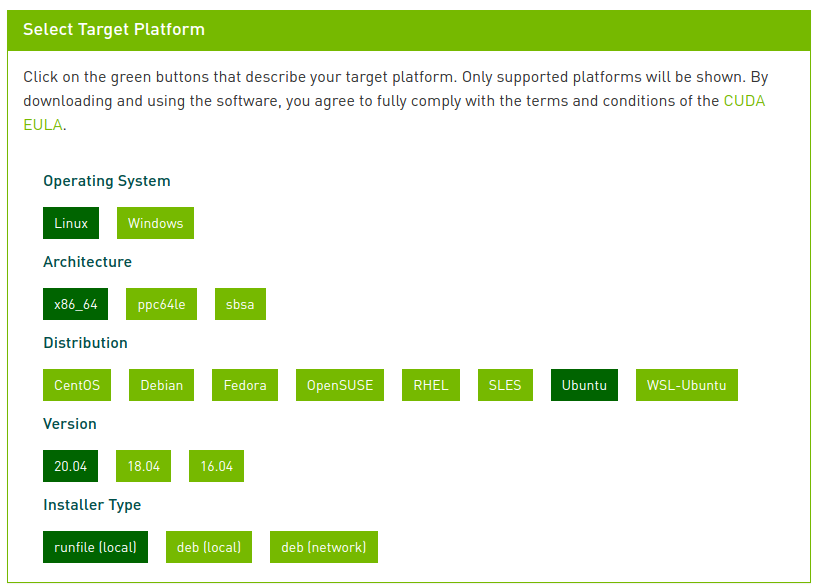
\includegraphics[width=9cm]{cuda1}
        \caption{CUDA 설치}
    \end{center}
\end{figure}
이후 지시사항에 따라 명령어를 입력하면 된다.
\begin{figure}[H]
	\begin{center}
        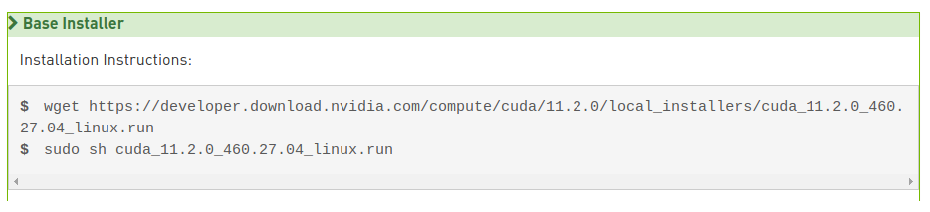
\includegraphics[width=12cm]{cuda2}
        \caption{CUDA 설치}
    \end{center}
\end{figure}


중간에 설치 프롬프트가 뜨는데, 스페이스 키를 눌러 드라이버는 설치에서 제외한다. 이후 설치를 진행하면 된다.
\begin{figure}[H]
	\begin{center}
        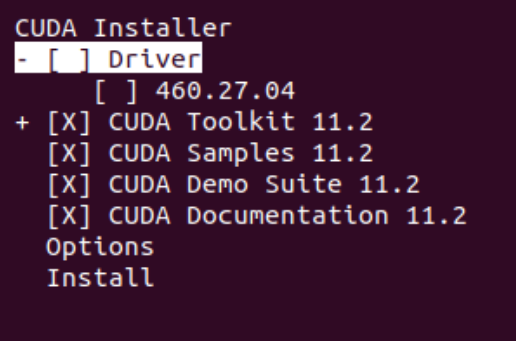
\includegraphics[width=5cm]{cuda3}
        \caption{CUDA 설치 - Drivers}
    \end{center}
\end{figure}

\subsection{환경변수 설정}
먼저 다음 명령어를 통해 CUDA를 환경변수에 등록한다. 11.2 자리에 다른 버전을 넣을 수도 있다.
\begin{lstlisting}
    $ sudo sh -c "echo 'export PATH=$PATH:/usr/local/cuda-11.2/bin' >> /etc/profile"

    $ sudo sh -c "echo 'export LD_LIBRARY_PATH=$LD_LIBRARY_PATH:/usr/local/cuda-11.2/lib64' >> /etc/profile"

    $ sudo sh -c "echo 'export CUDADIR=/usr/local/cuda-11.2' >> /etc/profile"

    $ source /etc/profile
\end{lstlisting}
이후 다음 명령어를 입력했을 때 CUDA 버전이 올바르게 출력된다면 설치 성공이다.
\begin{lstlisting}
    $ nvcc -V
\end{lstlisting}
\subsection{cuDNN 설치}
Nvidia Developer 사이트\href{https://developer.nvidia.com/cudnn}{(링크)}에 들어간다.
로그인 또는 회원가입 후 약관 및 서약에 동의하면 링크가 생긴다. 여기서 Archived cuDNN Releases에 들어가 cuDNN v8.1.1 (Feburary 26th, 2021), for CUDA 11.0,11.1 and 11.2를 다운로드 받는다.
\begin{figure}[H]
	\begin{center}
        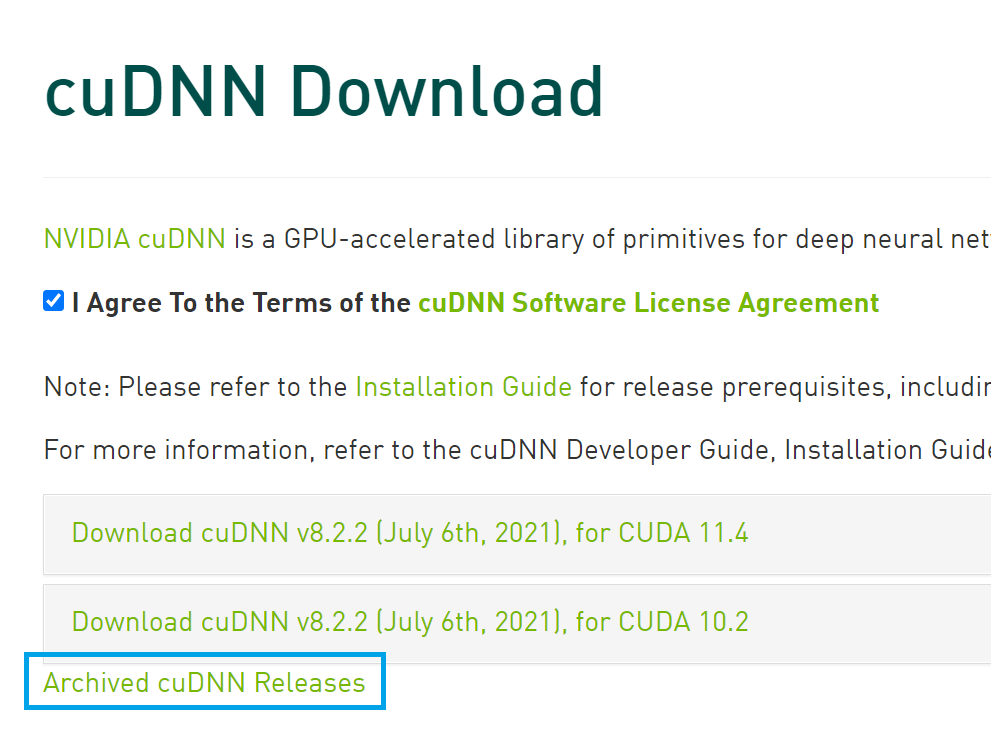
\includegraphics[width=12cm]{cudnn1}
        \caption{cuDNN 설치}
    \end{center}
\end{figure}

이 파일은 서버에서는 다운받을 수 없다. 따라서 sftp 등의 방법으로 서버에 업로드해야 한다. 이후 다음 명령어를 차례로 입력한다.
\begin{lstlisting}
    $ tar xvzf cudnn-11.2-linux-x64-v8.1.1*.tgz

    $ sudo cp cuda/include/cudnn* /usr/local/cuda/include

    $ sudo cp cuda/lib64/libcudnn* /usr/local/cuda/lib64

    $ sudo chmod a+r /usr/local/cuda/include/cudnn.h /usr/local/cuda/lib64/libcudnn*


    $ sudo ln -sf /usr/local/cuda-11.2/targets/x86_64-linux/lib/libcudnn_adv_train.so.8.1.1 /usr/local/cuda-11.2/targets/x86_64-linux/lib/libcudnn_adv_train.so.8

    $ sudo ln -sf /usr/local/cuda-11.2/targets/x86_64-linux/lib/libcudnn_ops_infer.so.8.1.1  /usr/local/cuda-11.2/targets/x86_64-linux/lib/libcudnn_ops_infer.so.8

    $ sudo ln -sf /usr/local/cuda-11.2/targets/x86_64-linux/lib/libcudnn_cnn_train.so.8.1.1  /usr/local/cuda-11.2/targets/x86_64-linux/lib/libcudnn_cnn_train.so.8

    $ sudo ln -sf /usr/local/cuda-11.2/targets/x86_64-linux/lib/libcudnn_adv_infer.so.8.1.1  /usr/local/cuda-11.2/targets/x86_64-linux/lib/libcudnn_adv_infer.so.8

    $ sudo ln -sf /usr/local/cuda-11.2/targets/x86_64-linux/lib/libcudnn_ops_train.so.8.1.1  /usr/local/cuda-11.2/targets/x86_64-linux/lib/libcudnn_ops_train.so.8

    $ sudo ln -sf /usr/local/cuda-11.2/targets/x86_64-linux/lib/libcudnn_cnn_infer.so.8.1.1 /usr/local/cuda-11.2/targets/x86_64-linux/lib/libcudnn_cnn_infer.so.8

    $ sudo ln -sf /usr/local/cuda-11.2/targets/x86_64-linux/lib/libcudnn.so.8.1.1  /usr/local/cuda-11.2/targets/x86_64-linux/lib/libcudnn.so.8

    $ sudo ldconfig
\end{lstlisting}
이후 다음 명령어를 입력했을 때 버전이 정확하게 출력되면 된다.
\begin{lstlisting}
    $ ldconfig -N -v $(sed 's/:/ /' <<< $LD_LIBRARY_PATH) 2>/dev/null | grep libcudnn
\end{lstlisting}
\section{Storage}
신서버를 구축하면서 15T짜리 디스크 레이드를 구성해야 되는 일이 생겼다. 이와 관련된 얘기들을 적을 예정. LVM groups가 무엇인가?, mount는 무엇인가?, 레이드는 무엇인가? 

    
\graphicspath{{./chap5/images/}}  
\chapter{Other}

\textbf{이 장은 서버의 다른 이용 방법들을 다룬다.}

\section{NewKOI}
Hydro랑 Vj4 번역 거의 했음
\section{CMS}

이건 37기 권준우가 적어둔 \href{https://github.com/gshslinuxintro/cslab.gs.hs.kr/tree/master/docs/cms}{문서(링크)}를 참고하자. 
\section{DB}
MySQL로 적는게 좋을듯?
\section{GCC}
To-do: cmake(?)
\section{Robocode}
To-do: x-11 디스플레이 포트포워딩, java 설치

    \appendix
        \chapter{Troubleshooting}
\section{Graphic Driver}
\subsection{nvidia-smi}
nvidia driver labrary mismatch~\\

cuda
\section{Storage}
dev1
\section{Python Environments}
pip, pip3, venv
\section{Jupyter}
config
\section{SSH}
sshd\_config
\section{Database}
mongodb, mariadb
\section{Nginx}
nginx.conf     % these are just test names as I didn't know what you'd want
        \chapter{GSHS CSLAB}
정보과 연구용 기기 목록
\begin{itemize}
    \item Nvidia RTX 2070 eGPU $\times$ 2
    \item Nvidia RTX 2080 Super eGPU $\times$ 1
    \item Nvidia RTC 3070 $\times$ 1 
    \item Intel NUC $\times$ 2
    \item 메인 서버.
    \item 구서버 (테스트용 서버)
\end{itemize}
    
        
\chapter{Contributors}

37st (Version1) : 19007 권준우, 19011 김도영, 19032 노현서, 19042 박영민


38st (Version2) : 20059 송혁중 

{\backmatter
    % Bibliography
    \if@openright\cleardoublepage\else\clearpage\fi
    \bibliographystyle{gs-plainnat} %% specific plainnat does not show url for articles
    {\footnotesize\bibliography{chap1/introduction_biblio,chap2/background_and_lit_overview_biblio}}
	\printindex
}

\end{document}

%%% The End %%%